\documentclass{vgtc}
\graphicspath{{figs/}}
\usepackage{fontspec}
\setmainfont{texgyretermes}[Extension=.otf, UprightFont=*-regular, BoldFont=*-bold, ItalicFont=*-italic, BoldItalicFont=*-bolditalic]
\usepackage{booktabs}

\onlineid{0}
\vgtccategory{Research}
\vgtcinsertpkg

\title{LLM Chart Judges Reward Labels, Not What Audiences Upvote}

\newif\ifanonymous\anonymoustrue
\ifanonymous
  \author{Anonymous Author(s)\\ \scriptsize Affiliation withheld for review}
\else
  \author{Rahul Chaudhary\\ \scriptsize Independent Researcher, New York, NY, USA}
\fi

\teaser{
  \centering
  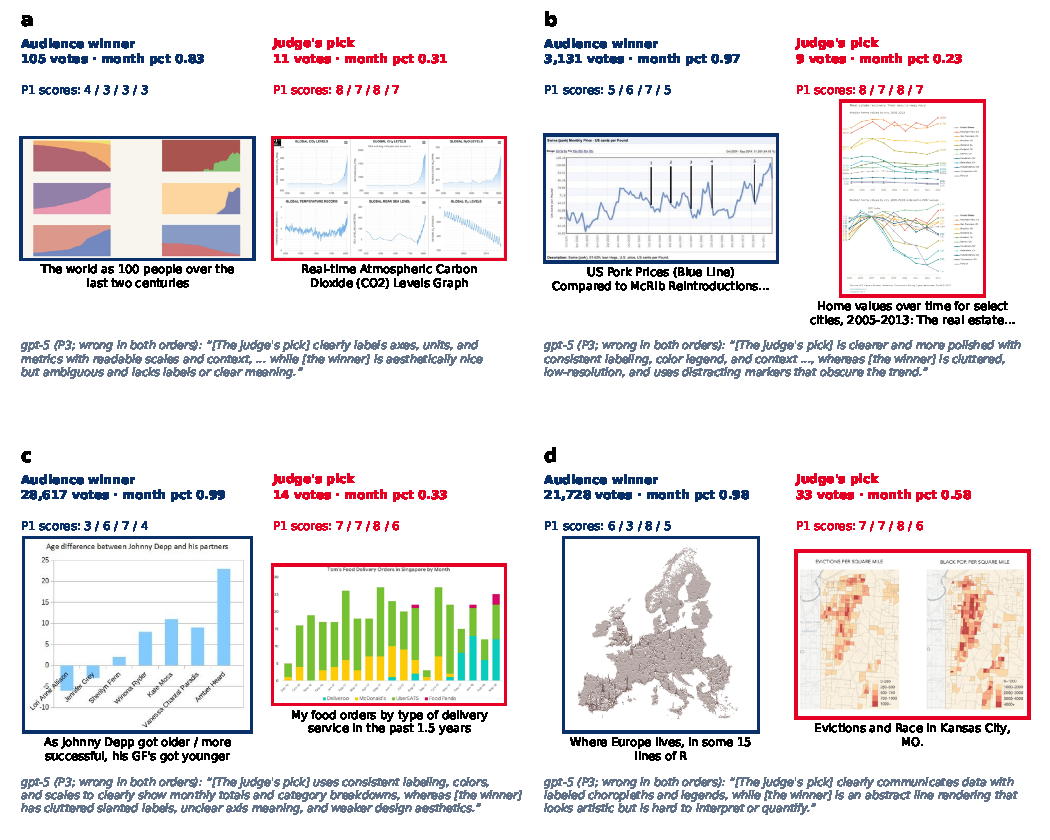
\includegraphics[width=\linewidth, alt={Four pairs of charts from r/dataisbeautiful. In each pair the audience strongly preferred the left chart, but every LLM judge scored the right chart higher, citing labels, legends and clarity.}]{fig5_examples.pdf}
  \refstepcounter{figure}\label{fig:teaser}
  \par\vspace{2pt}{\captionfonts Figure~\thefigure: Four pairs posted in the same week with the same chart type, where the audience winner (navy) received 9--2{,}000$\times$ the votes of the chart the judges preferred (red). P1 scores are from gpt-5 / Claude Haiku 4.5 / Gemini 2.5 Flash / Claude Sonnet 5.5. In 15 of 16 judge--pair cases the judge scores the loser higher, and the remaining case is a tie. The quotes come from gpt-5's pairwise prompt, which picked the loser in both A/B orders. They are verbatim except that ``Chart A/B'' is replaced by a bracketed referent. The judges reward labels, legends, and annotation. The audience rewards a striking idea (a), a joke (b), a celebrity topic (c), and minimal, artful form (d).\par}
}

\abstract{Multimodal LLMs now score charts that AI agents generate, and they are validated by agreement with expert ratings. We test whether such judges agree with what a public audience rewards. From 34{,}556 cleaned r/dataisbeautiful charts (2012--2025) we build 2{,}000 pairs of charts posted in the same week with the same chart type, where one received at least five times the other's votes. An image-blind baseline that sees only the title and posting time picks the winner 59.1\% of the time. In a pre-registered equivalence analysis on identical pairs, three judges (gpt-5, Claude Haiku 4.5, Gemini 2.5 Flash) score 55.4--57.6\%, and the frontier Claude Sonnet 5.5 scores 57.8\% on 1{,}000 pairs. For every judge we reject an advantage of four points or more over the baseline (one-sided $p\le0.002$); the upper 90\% confidence bounds lie between $-0.3$ and $+1.5$ points. Haiku is significantly worse than the baseline. Judge scores still add significant independent signal on top of it, so the judges are informative, but none outperforms titles and timing. The gap has a consistent direction. The same holistic scores correlate 0.44--0.49 with expert ratings but only 0.08--0.13 with audience vote percentile. Every judge rewards text-heavy charts ($+0.32$ to $+0.51$ per SD of OCR word count) while the audience does not ($-0.02$), and one judge reverses its pairwise choice on 53\% of pairs when the order is swapped. Expert alignment does not transfer to audiences.}

\keywords{LLM-as-a-judge, visualization quality, audience engagement, equivalence testing, Reddit.}

\begin{document}

\firstsection{Introduction}
\maketitle

Multimodal LLMs increasingly act as judges of charts produced by AI agents, in benchmarks, challenges, and product evaluation pipelines. A judge is usually validated against experts. VisJudge-Bench~\cite{xie2026visjudge} reports that GPT-5 correlates 0.428 with expert quality ratings on 3{,}090 visualizations, and a fine-tuned 7B model reaches 0.687.

Many charts, however, are made for a public audience, and nobody has tested whether these judges reward what that audience rewards. Measuring audience preference is hard because raw engagement mostly reflects timing, title, and topic~\cite{kauer2021public}. r/dataisbeautiful has 13 years of charts with vote counts, packaged as beautiVis~\cite{lin2026beautivis}. We compare charts only with close neighbors: two charts posted in the same ISO week, with the same chart type, where one received at least five times the other's votes. We ask whether a judge picks the audience winner more often than a baseline that never sees the image.

Our contributions are:
\begin{itemize}
\item a controlled pairwise protocol and an image-blind baseline for measuring the audience alignment of chart judges;
\item a pre-registered equivalence analysis showing that four LLM judges, including a frontier model, do not beat titles and timing by 4 points or more (and one is significantly worse), even though they reach expert-level agreement with the same prompt;
\item evidence that judges systematically reward text-heavy, labeled charts, a preference the audience does not share, and that position bias makes one judge's pairwise choices unreliable.
\end{itemize}

\section{Related Work}
\textbf{LLMs as visualization judges.} VisJudge-Bench~\cite{xie2026visjudge} scores charts on six expert dimensions (fidelity, expressiveness, aesthetics) and finds moderate model--expert agreement. Seto et al.~\cite{seto2026literacy} report that current frontier models exceed human scores on a visualization-literacy test but still struggle to judge whether a chart is misleading without leading prompts. Panda~\cite{panda2026personas} prompts LLMs to adopt literacy-stratified personas and benchmarks them against published human responses to literacy items and aesthetic ratings. Li et al.~\cite{li2026beauty} compare LLM and human choices of the most pleasing network layout, and Jeon et al.~\cite{jeon2026llmsee} compare how humans and LLMs describe the same charts. All of these use experts, lab participants, or study instruments. We use votes from a public audience. Position bias in pairwise LLM judging is well documented for text~\cite{zheng2023judging}, and we measure it for charts.

\textbf{Audiences on r/dataisbeautiful.} Kauer et al.~\cite{kauer2021public} found that comments on the subreddit mostly discuss topic and insight, and only rarely design. beautiVis~\cite{lin2026beautivis} provides 52{,}836 visualization posts with GPT-4o chart-type labels mapped to MASSVIS-style categories~\cite{borkin2013memorable}.

\section{Data, Pairs, and Baseline}
\textbf{Cleaning.} From the 52{,}836 beautiVis rows we removed:
\begin{itemize}
\item blank images (148, mostly video thumbnails);
\item posts with an empty or ``Other'' chart type (6{,}449);
\item images whose short side is under 300\,px (1{,}806);
\item posts with fewer than 5 votes (8{,}505), mostly removed or spam posts;
\item near-duplicate images (1{,}372; perceptual-hash distance $\le$2, keeping the earliest post).
\end{itemize}
Groups of three or more near-identical images with unrelated titles are link previews, so we removed them entirely. No rule looks at votes. This leaves 34{,}556 posts, 31{,}542 of them with a single chart type. Supplement S1 gives the details.

\textbf{Pairs.} We bucket posts by ISO week $\times$ chart type and form \emph{clear} pairs, in which the winner has at least 5 times the loser's votes and at least 50 votes. Each bucket contributes at most three pairs, and each post is used at most once. Pairs are drawn round-robin over years, so all years from 2012 to 2025 appear, and no chart type exceeds 25\%. The display order is randomized. This gives 2{,}000 pairs, with a median vote ratio of 32.

\textbf{Image-blind baseline.} An L2 logistic regression predicts the winner from the difference between the two posts' features: title TF-IDF, title length, an \texttt{[OC]} (original content) flag, posting hour, and weekday. Folds are grouped by month, and we use out-of-fold predictions. The baseline picks the winner on 59.1\% of the 2{,}000 pairs (95\% CI 57.0--61.2).

\section{Judges and Analysis Plan}
Every judge sees the same standardized JPEG (white background, long side $\le$1536\,px) and never sees the title. The primary prompt, P1, asks for a holistic 1--10 score for clarity, design, and visual appeal. A pair is credited 1 if the audience winner scores higher, 0.5 on a tie, and 0 otherwise.

The three main judges each score all 4{,}000 images: gpt-5 (minimal reasoning), Claude Haiku 4.5, and Gemini 2.5 Flash (temperature 0 for both). Claude Sonnet 5.5 (low effort) is the frontier judge and scores the first 1{,}000 pairs. Of 14{,}000 P1 requests, one failed to parse; it is counted as a tie. On 150 VisJudge-Bench items, our rubric-prompt setup gives gpt-5 a Pearson $r$ of 0.414 against expert scores, matching the published 0.428 (Supplement S3).

We wrote the analysis plan before running the 2{,}000-pair evaluation. For each judge, the test is a two one-sided tests (TOST) equivalence test of the paired accuracy difference (judge minus baseline) with a margin of $\pm$4 points and $\alpha=0.05$. A judge is called equivalent when the 90\% bootstrap CI (10{,}000 resamples) lies inside the margin. As a robustness check we repeat the analysis on the 1{,}500 pairs that no judge had seen during development. Position bias is measured separately with a pairwise prompt that is run in both A/B orders.

\section{Results}
\begin{table}[tb]
  \caption{P1 accuracy on identical clear pairs. $\Delta$: judge minus baseline, in points, with its 90\% bootstrap CI. $p_{>+4}$: one-sided test that the judge beats the baseline by 4 points or more. LR $p$: likelihood-ratio test of adding the judge's score difference to the baseline model. $^\dagger$Sonnet is compared on the first 1{,}000 pairs, where the baseline scores 59.6\%.}
  \label{tab:main}
  \scriptsize
  \centering
  \setlength{\tabcolsep}{3pt}
  \resizebox{\columnwidth}{!}{%
  \begin{tabular}{@{}lrcrcc@{}}
  \toprule
  Judge (P1) & $n$ & Accuracy (95\% CI) & $\Delta$ [90\% CI] & $p_{>+4}$ & LR $p$ \\
  \midrule
  Image-blind baseline & 2{,}000 & .591 (.570--.612) & -- & -- & -- \\
  gpt-5 & 2{,}000 & .564 (.544--.582) & $-2.8$ [$-5.1$, $-0.3$] & $2\!\times\!10^{-6}$ & $<10^{-4}$ \\
  Claude Haiku 4.5 & 2{,}000 & .554 (.537--.572) & $-3.7$ [$-5.9$, $-1.3$] & $3\!\times\!10^{-8}$ & $<10^{-4}$ \\
  Gemini 2.5 Flash & 2{,}000 & .576 (.558--.593) & $-1.5$ [$-3.9$, $+0.9$] & $4\!\times\!10^{-5}$ & $<10^{-4}$ \\
  Claude Sonnet 5.5$^\dagger$ & 1{,}000 & .578 (.551--.604) & $-1.9$ [$-5.2$, $+1.5$] & .002 & -- \\
  \bottomrule
  \end{tabular}}
\end{table}

\begin{figure}[tb]
  \centering
  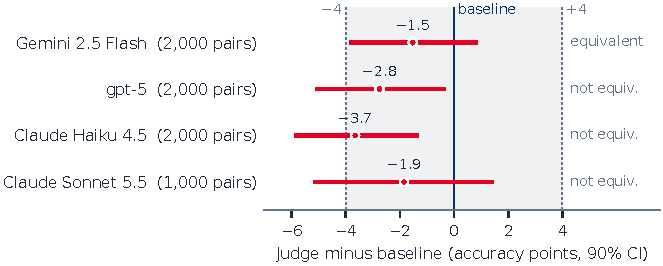
\includegraphics[width=\columnwidth, alt={Forest plot of judge-minus-baseline accuracy with 90 percent confidence intervals and a shaded plus-or-minus four point margin. All intervals end below plus 1.5 points.}]{fig7_tost.pdf}
  \caption{Pre-registered equivalence test. The shaded band is the $\pm$4-point margin. No judge's 90\% CI extends above $+1.5$ points.}
  \label{fig:tost}
\end{figure}

\textbf{RQ1: No judge beats titles and timing.} No judge beats the image-blind baseline by 4 points or more (\cref{tab:main}, \cref{fig:tost}). Every point estimate is below it, and every upper 90\% bound lies between $-0.3$ and $+1.5$ points. For every judge we reject an advantage of four points or more ($p\le0.002$). Under the pre-registered two-sided rule, Gemini Flash is equivalent to the baseline (TOST $p=0.039$). gpt-5 and Haiku are inconclusive only because they may be more than four points \emph{worse}; Haiku is significantly below the baseline (95\% CI $[-6.4, -0.9]$). The frontier judge does not close the gap. Sonnet 5.5 is equivalent to gpt-5 and to Flash on its 1{,}000 pairs (differences $+0.7$ and $+0.5$ points; TOST $p=0.004$ and $0.002$). On the 1{,}500 pairs unseen during development the estimates are almost unchanged ($-2.8$, $-3.2$, and $-1.4$ points).

The judges are not uninformative, though. Adding a judge's score difference to the baseline's out-of-fold logit improves the fit for every judge (likelihood-ratio $\chi^2$ of 17--40, $p<10^{-4}$), but AUC rises only from 0.623 to between 0.634 and 0.649. The judges see something that titles and timing miss. As predictors of votes, however, they are weaker than titles and timing.

\textbf{Expert alignment does not transfer.} Both comparisons use the same P1 scores and the same rank correlation (Spearman $\rho$). On 150 VisJudge-Bench items, judge scores correlate $\rho=0.44$--0.49 with expert ratings. On the 4{,}000 audience images they correlate only $\rho=0.08$--0.13 with each post's vote percentile within its month (Sonnet: 0.12).

\begin{figure}[tb]
  \centering
  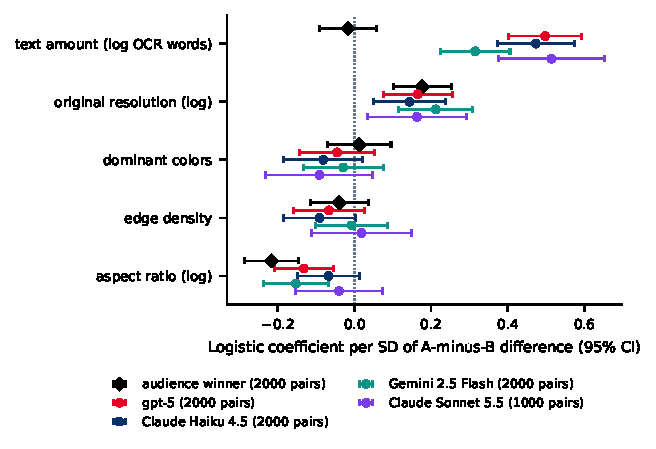
\includegraphics[width=\columnwidth, alt={Coefficients for five image features. For text amount the audience coefficient is near zero while all four judges are between 0.3 and 0.5. For the other features audience and judges overlap.}]{fig8_bias_all.pdf}
  \caption{Image features that predict the audience winner (black) and each judge's P1 pick. Coefficients come from logistic regressions on the A-minus-B feature difference. Text amount is the only feature on which judges and audience clearly diverge.}
  \label{fig:bias}
\end{figure}

\textbf{RQ2: Judges reward text; the audience does not.} We computed five features per image (OCR word count, dominant-color count, edge density, aspect ratio, and original resolution) and fit logistic regressions on the A-minus-B feature differences, separately for the audience winner and for each judge's pick (\cref{fig:bias}). Four of the five features have overlapping coefficients for judges and audience. Text is the exception: every judge favors the chart with more words ($+0.32$ to $+0.51$ per SD, SE 0.05--0.07), while the audience coefficient is $-0.02$ (SE 0.04). The judges' stated reasons match this pattern (\cref{fig:teaser}). They praise ``consistent labeling,'' ``color legend,'' and ``readable scales,'' and penalize charts that are ``abstract'' or ``ambiguous.'' The audience winners in \cref{fig:teaser} are a striking idea, a joke, a celebrity topic, and a minimalist map without a single label. In 15 of the 16 judge--pair cases, the judge scores the less-voted chart higher; the remaining case is a tie.

\textbf{RQ3: Position bias.} With a pairwise prompt (``Which is the better visualization?'') shown in both orders, gpt-5 and Haiku change their answer on 18\% of 250 pairs. Gemini Flash changes its answer on 53\% of 500 pairs and picks whichever chart is shown first 77\% of the time. Single-order pairwise results from such a judge are close to arbitrary. Pairwise accuracy is no higher than P1 accuracy for any judge (Supplement S2).

\section{Discussion}
The judges match published expert-alignment numbers, yet none predicts audience votes better than a model that reads only titles and timestamps; the best point estimate is 1.5 points below it. On the first 250 pairs, for example, gpt-5 picks the winner 62.8\% of the time from the two titles alone and 63.6\% with the charts in view (Supplement S2). Whatever the judges know about appeal seems to come from topic rather than design. The divergence has a direction. Judges apply a checklist of labeling and annotation, and many charts the audience rewards would fail that checklist. For anyone scoring chart-generating agents, an LLM judge is evidence of conformance to conventions, not of engagement. Systems that optimize for an audience need audience data or an audience-calibrated judge. Pairwise judging should always be run in both orders.

\section{Limitations}
\begin{itemize}
\item \textbf{One noisy audience.} Votes are noisy, and r/dataisbeautiful is one community whose rules shape what gets posted.
\item \textbf{Lopsided pairs.} Clear pairs are very unequal, and some losers may be low-effort posts. Such losers should be easy to spot, which would favor the judges rather than the baseline.
\item \textbf{Indirect evidence for topics.} Our suggestion that audiences respond to topic rests on the strength of the title baseline and on prior work~\cite{kauer2021public}; we did not code topics directly.
\item \textbf{Models and budget.} Budget limits kept Sonnet 5.5 to 1{,}000 pairs. We did not test an expert-tuned judge (VisJudge-7B), and we use beautiVis's GPT-4o chart-type labels.
\end{itemize}

\section*{Supplemental Materials}
\label{sec:supplemental_materials}
The supplement contains:
\begin{itemize}
\item S1: cleaning details and the deviations from our original plan;
\item S2: rubric (P2) and pairwise (P3) prompts, the title-only control, and close pairs;
\item S3: calibration on VisJudge-Bench;
\item S4: memorization checks;
\item S5: the pre-registration text.
\end{itemize}
We release code, prompts, post identifiers and permalinks, all raw judge responses with token usage, and all analysis tables. Images are not redistributed.

\section*{Figure Credits}
\label{sec:figure_credits}
\Cref{fig:teaser} reproduces eight charts posted to r/dataisbeautiful, retrieved through beautiVis~\cite{lin2026beautivis}, and shown here for commentary. Credits, as Reddit user and post ID: (a) u/RightFloor \texttt{5jk2ub}, u/Sourcecode12 \texttt{5jn2mu}; (b) u/OMGLMAOWTF\_com \texttt{2ionwm}, u/marriedacarrot \texttt{2it1p7}; (c) u/Smart\_Ass\_Pawn \texttt{8awx8s}, u/tomeczak \texttt{8awz4p}; (d) u/halhen \texttt{671s4d}, u/AbeDrinkin \texttt{66ifjl}. Each post is at \texttt{reddit.com/r/dataisbeautiful/comments/<id>}.

\bibliographystyle{abbrv-doi}
\bibliography{refs}
\end{document}
